%!TEX root = ../thesis.tex
\chapter{Fundamentals}
\label{ch:fundamentals}

\section{Computer Vision}
\todo{Nochmal neu formulieren?}
Computer Vision ist ein Teilbereich der künstlichen Intelligenz, der eng mit der Bildverarbeitung und dem maschinellen Lernen verknüpft ist. Dabei wird die Rohdatenerfassung durch Verfahren erweitert, die digitale Bildverarbeitung, Mustererkennung, maschinelles Lernen und Computergrafik kombinieren. Ziel ist es, Maschinen die menschliche Fähigkeit zu verleihen, aus Bildern Informationen zu extrahieren und zu interpretieren \citep{Wiley2018}. Zur Informationsgewinnung und zur Simulation menschlicher visueller Wahrnehmung werden Algorithmen sowie optische Sensoren eingesetzt \citep{Matiacevich2013}. Es lässt sich zwischen Bildbeschaffung und Bildanalyse unterscheiden. Wichtige Komponenten der Bildanalyse sind unter anderem:
\begin{itemize}
    \item \textbf{Bilderzeugung:} Das Speichern eines Objekts als digitales Bild.
    \item \textbf{Bildverarbeitung:} Verbesserung der Bildqualität zur Erhöhung des Informationsgehalts.
    \item \textbf{Bildsegmentierung:} Trennung des Objekts vom Hintergrund.
    \item \textbf{Bildvermessung:} Ermittlung signifikanter Bildpunkte (sogenannter Features).
    \item \textbf{Bildinterpretation:} Ableitung semantischer Informationen aus den Bilddaten \citep{Mery2013}. 
\end{itemize}



%\section{Machine Learning}
%\todo{Nochmal neu formulieren?}


% Im Bereich des maschinellen Lernens lassen sich grundsätzlich drei Hauptarten unterscheiden: das überwachte Lernen (supervised learning), unüberwachte Lernen (unsupervised learning) und das Reinforcement Learning.

% Beim überwachten Lernen liegt ein klar definiertes Ziel vor, das mithilfe gelabelter Trainingsdaten erlernt werden soll. Innerhalb dieses Ansatzes unterscheidet man vor allem zwischen zwei Formen: Klassifikation und Regression. Bei der Klassifikation geht es darum, Eingabedaten einer vordefinierten Anzahl an Klassen korrekt zuzuordnen. Die Trainingsdaten enthalten dafür bereits bekannte Klassenzugehörigkeiten, anhand derer das Modell lernen kann, auch neue, unbekannte Eingaben richtig einzuordnen.Im Gegensatz dazu steht die Regression, bei der das Ziel die Vorhersage eines kontinuierlichen Wertes ist. Die Ausgabe wird dabei durch verschiedene Eingabegrößen beeinflusst und basiert auf einer zugrunde liegenden funktionalen Beziehung zwischen Ein- und Ausgabegrößen \cite{Braga-Neto2020}.

% Beim unüberwachten Lernen hingegen erhält der Algorithmus Daten ohne vorgegebene Labels. Ziel ist es, eigenständig Strukturen, Muster oder Auffälligkeiten in den Daten zu identifizieren und Gruppenbildungen (Cluster) zu erkennen \cite{Braga-Neto2020}.

% Das sogenannte Reinforcement Learning stellt einen weiteren Lernansatz dar, bei dem ein Modell durch Interaktion mit seiner Umgebung lernt. Es wird dabei durch ein Belohnungssystem gesteuert: Für erwünschte Handlungen erhält es positive Rückmeldungen, während unerwünschtes Verhalten bestraft wird. So entwickelt das Modell schrittweise eine Strategie zur Optimierung seines Verhaltens \cite{Braga-Neto2020}.

%In den folgenden Abschnitten wird der Fokus auf die Detektion und Klassifikation als Teilgebiet des überwachten Lernens gelegt.


\section{Machine and Deep Learning}


Maschinelles Lernen beschreibt einen Ansatz in der Informatik, bei dem Algorithmen auf Basis von vorhandenen Daten selbstständig Muster erkennen, um ein definiertes Ziel zu erreichen – etwa die Klassifikation von Informationen. Im Gegensatz zu traditionellen Algorithmen, die feste, vom Menschen vorgegebene Regeln befolgen, entwickelt ein lernfähiger Algorithmus eigene Verarbeitungsstrategien. Die Entscheidungslogik entsteht dabei nicht durch manuelle Programmierung, sondern durch die Analyse von Daten und das Erkennen wiederkehrender Strukturen \cite{Shetty2022}.Der Begriff „Lernen“ bezieht sich allgemein auf den Prozess, bei dem Wissen oder Fähigkeiten durch Erfahrung, Versuch und Irrtum, Anleitung oder Beobachtung erworben werden. Übertragen auf den maschinellen Kontext bedeutet dies, dass Maschinen durch wiederholte Analyse und Rückmeldung in der Lage sind, aus Beispielen zu generalisieren und neue, unbekannte Daten zu verarbeiten. Maschinelles Lernen kann daher als rechnergestützte Nachbildung menschlicher Lernprozesse verstanden werden, bei der Algorithmen in der Lage sind, abstrahierte Regeln aus Rohdaten zu entwickeln und auf neue Situationen anzuwenden \cite{Fischer1999, Braga-Neto2020}. Diese Fähigkeit eröffnet neue Möglichkeiten bei der Lösung komplexer Probleme, die sich mit konventionellen, regelbasierten Methoden nur schwer oder gar nicht bearbeiten lassen \cite{Goodfellow-et-al-2016}.

\begin{figure}[h]
    \centering
    \includegraphics[width=0.6\textwidth, clip, trim= 2cm 8cm 2cm 2cm]{svg-inkscape/ML_and_DL_svg-tex.pdf}
    \caption{Overview over Artificial Intelligence, Machine Learning and Deep Learning. \cite{Alzubaidi2021}}
    \label{fig:ML_andD_L}
\end{figure}

\acrfull{DL} ist ein Teilgebiet des maschinellen Lernens (s. Fig. \ref{fig:ML_andD_L}), dessen Funktionsweise von den neuronalen Prozessen im menschlichen Gehirn inspiriert ist. Es simuliert den Informationsverarbeitungsprozess, wie er in zentralen sensorischen Regionen des Gehirns abläuft. Im Gegensatz zu klassischen regelbasierten Verfahren arbeitet \acrshort{DL} nicht mit strikt von Menschen entworfenen Regeln, sondern nutzt große Datenmengen, um Muster zu erkennen und Eingaben auf spezifische Eigenschaften hin zu analysieren. Charakteristisch ist dabei die Verwendung zahlreicher Schichten \acrfullpl{ANN}, in denen jede Schicht die zugelieferten Informationen in einer einzigartigen Form interpretiert. Während herkömmliche Techniken des maschinellen Lernens meist auf eine Trennung von Pre-Processing, Feature Extraction, Feature Selection, Learning und Classification angewiesen sind, kann \acrshort{DL} diese Schritte teilweise automatisieren und in einem einzigen End-to-End-Prozess zusammenführen. Dadurch werden sowohl das Lernen von Feature Sets für mehrere Aufgaben als auch Klassifikation in einem Schritt ermöglicht \cite{Alzubaidi2021}. 

Zu den zentralen Vorteilen von \acrshort{DL} zählen seine universelle Anwendbarkeit in verschiedensten Bereichen, die Robustheit durch die automatisierte Extraktion optimierter Merkmale anstelle handgefertigter Features, die Fähigkeit zur Verallgemeinerung über verschiedene Datentypen hinweg – beispielsweise durch Transferlernen, was besonders in Szenarien mit geringen Datenmengen relevant ist – sowie eine hohe Skalierbarkeit, da Netzwerke unkompliziert durch zusätzliche Knoten erweitert werden können. Grundsätzlich lassen sich DL-Ansätze in drei Kategorien unterteilen: überwachtes, semi-überwachtes und unüberwachtes Lernen\cite{Alzubaidi2021}.  

Beim überwachten Lernen (Supervised Learning) erhält ein Algorithmus eine Sammlung von Eingaben und den zugehörigen Ausgaben. Ein intelligenter Agent schätzt eine Ausgabe $\hat{y}_t = f(x_t)$ für eine Eingabe $x_t$ und berechnet den Verlust $tz(\hat{y}_t, y_t)$ als Abweichung zur bekannten Zielausgabe $y_t$. Durch wiederholte Anpassung der Netzwerkparameter wird das Modell sukzessive optimiert, bis die Schätzungen mit den tatsächlichen Ausgaben übereinstimmen. Typische Architekturen in diesem Bereich sind \acrfullpl{RNN}, \acrfullpl{CNN} und \acrfullpl{DNN}. Im semi-überwachten Lernen werden Datensätze verwendet, die nur teilweise gelabelt sind. Dies reduziert die benötigte Menge an Trainingsdaten mit Annotationen, birgt jedoch die Gefahr, dass irrelevante Eingangsmerkmale zu falschen Klassifikationen führen können. Ein klassisches Anwendungsbeispiel ist die Textklassifikation. Im unüberwachten Lernen schließlich werden gänzlich ungelabelte Daten genutzt, um signifikante Merkmale oder innere Strukturen in den Daten zu identifizieren. Hierbei kann das Modell Cluster oder Zusammenhänge entdecken, jedoch liefert dieser Ansatz keine präzisen Informationen über die Sortierung der Daten und ist zudem rechenintensiv \cite{Alzubaidi2021}.  

Innerhalb der Vielzahl an Netzarchitekturen haben sich \acrshortpl{CNN} als die wohl bekannteste und am häufigsten genutzte Variante etabliert. Inspiriert von biologischen Neuronenstrukturen identifizierte \cite{Goodfellow-et-al-2016} drei zentrale Vorteile von CNNs: gleichwertige Darstellungen, spärliche Interaktionen sowie eine effiziente Parameternutzung durch Weight Sharing. Eine Eingabe $x$ wird in den Schichten eines CNN durch drei Dimensionen repräsentiert: Höhe, Breite und Tiefe, wobei die Tiefe der Anzahl der Bildkanäle entspricht. In den Faltungsschichten (Convolutional Layers) werden Filter bzw. Kernel $k$ mit Dimensionen $n \times n \times q$ angewandt, die lokale Verbindungen und Feature Maps $h^k$ erzeugen \cite{Alzubaidi2021}. % Die Berechnung erfolgt dabei über das Punktprodukt zwischen Eingabe und Gewichtsmatrix:  
% \begin{equation}
% h^k = f(W^k \ast x + b^k).
% \end{equation}
Darauf folgt ein Downsampling der Feature Maps in sogenannten Pooling-Schichten, das die Anzahl der Netzparameter reduziert, den Trainingsprozess beschleunigt und Überanpassung (Overfitting) entgegenwirkt. Pooling-Operationen wie Max- oder Average-Pooling aggregieren lokale Regionen einer Feature Map, bevor die abstrahierten Merkmale in \acrfullpl{FCL} zusammengeführt werden. Die finale Klassifikation wird in der Ausgabeschicht häufig mit einem Klassifikator wie der \acrfull{SVM} realisiert. CNNs zeichnen sich durch bessere Generalisierung, Verhinderung von Overfitting durch Weight Sharing, flexible Nutzung extrahierter Merkmale und einfache Skalierbarkeit aus. Zu den zentralen Komponenten einer \acrshort{CNN}-Architektur gehören Convolutional Layers mit trainierbaren Filtern, Pooling Layers zur Dimensionsreduktion, Aktivierungsfunktionen wie \acrfull{ReLU} zur Einführung von Nichtlinearität, \acrshortpl{FCL} für die Merkmalsaggregation sowie Loss-Funktionen, die den Unterschied zwischen vorhergesagten und tatsächlichen Werten messen und für die Parameteroptimierung genutzt werden \cite{Alzubaidi2021}. \todo{Detaillierte Convolutional Operation noch einfügen}

\subsection{Backpropagation}

Der Lernprozess in Deep-Learning-Netzen basiert auf dem Prinzip der Backpropagation \cite{Goodfellow-et-al-2016}. Dabei wird zunächst in einer Vorwärtsphase (Forward Propagation) die Eingabe $x$ durch das Netzwerk propagiert, sodass am Ende die Ausgabe $y$ resultiert. Anschließend werden die Fehler durch Rückwärtspropagation (Backpropagation) schrittweise durch das Netz zurückgeführt, um Gradienten zu berechnen, die zur Aktualisierung der Gewichte genutzt werden. Dieses Verfahren ermöglicht eine effiziente Optimierung tiefer Netzwerke, stößt jedoch bei sehr tiefen Architekturen auf zwei zentrale Probleme: das Vanishing-Gradient-Problem und das Exploding-Gradient-Problem \cite{Alzubaidi2021}.  

\subsection{Vanishing-Gradient-Problem}

Das Vanishing-Gradient-Problem tritt auf, wenn die Gradienten in tiefen Netzen während der Backpropagation exponentiell kleiner werden und somit keine signifikanten Gewichtsaktualisierungen mehr möglich sind. Dies kann im Extremfall dazu führen, dass ein Netz das Lernen vollständig einstellt. Typische Ursachen sind die Verwendung von Aktivierungsfunktionen mit kleinen Ableitungen (wie Sigmoid oder Tanh) oder sehr tiefe Netze mit vielen Schichten. Mögliche Gegenmaßnahmen sind die Verwendung von Aktivierungsfunktionen wie \acrshort{ReLU}, Batch-Normalisierung zur Stabilisierung der Eingaben oder schnellere Hardware, die ein Training mit komplexeren Architekturen ermöglicht \cite{Alzubaidi2021}.  

\subsection{Exploding-Gradient-Problem}

Das Exploding-Gradient-Problem stellt den gegenteiligen Fall dar: hier wachsen die Gradienten während der Rückpropagation exponentiell an, was zu extrem hohen Gewichtsaktualisierungen, Instabilität und im schlimmsten Fall zu \acrfullpl{NaN-Value} (Werte, die undefiniert oder nicht darstellbar sind) führt. Gelöst werden kann dies etwa durch Regularisierungstechniken, angepasste Netzwerkarchitekturen oder Gradient Clipping \cite{Alzubaidi2021}.  

\subsection{Overfitting}
\label{subsec:overfitting}

\begin{figure}[h]
    \centering
    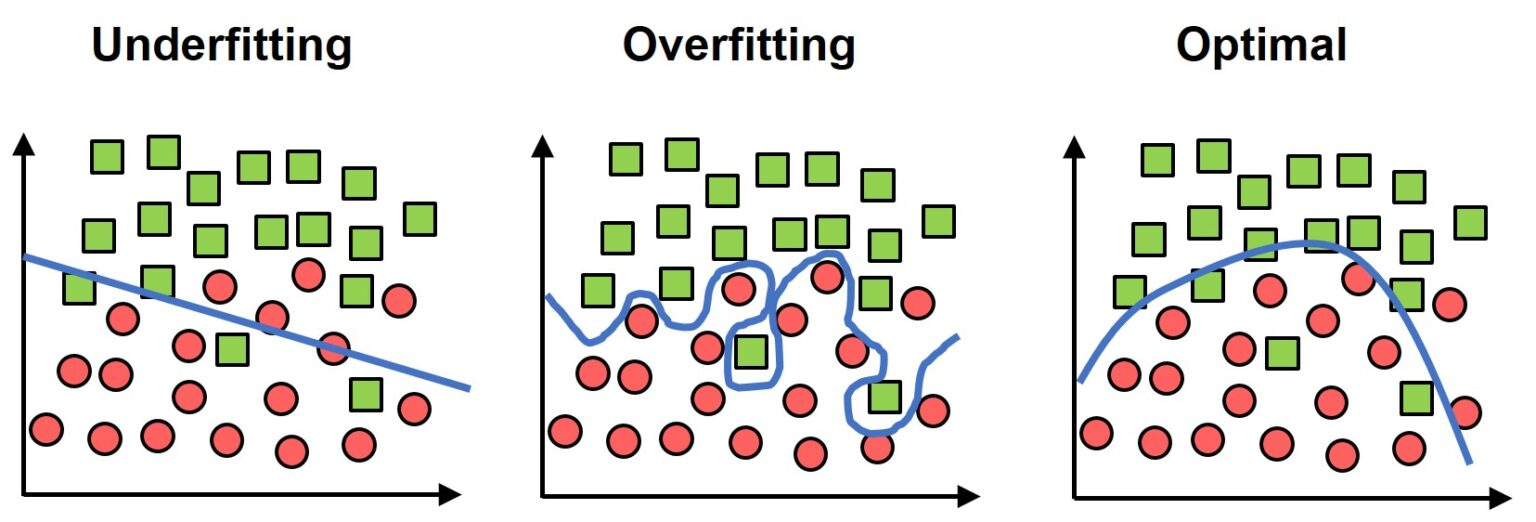
\includegraphics[width=0.8\textwidth]{images/011Fundamentals/overfitting.jpg}
    \caption{Underfitting, Overfitting and Optimal at Deep Learning Trainings. \cite{overfitting_pic} }
    \label{fig:overfitting}
\end{figure}


Ein zentrales Problem beim Training tiefer neuronaler Netze stellt das Overfitting dar (vgl. Abb. \ref{fig:overfitting}). In diesem Fall passt sich das Modell zu stark an die Trainingsdaten an: Es erzielt dort eine hohe Genauigkeit, während die Leistung auf unabhängigen Testdaten deutlich abnimmt. Das Gegenphänomen ist das Underfitting, bei dem die zugrunde liegende Datenstruktur nicht hinreichend erfasst wird und das Modell folglich sowohl im Trainings- als auch im Testdatensatz unzureichende Ergebnisse liefert. Ziel ist daher die Entwicklung eines Modells, das die relevanten Muster der Trainingsdaten adäquat erlernt und gleichzeitig eine hohe Generalisierungsfähigkeit gegenüber unbekannten Daten aufweist \cite{overfitting_pic}.\\
Die hohe Anzahl an Parametern in tiefen Netzen erhöht die Wahrscheinlichkeit, dass ein Modell die Trainingsdaten übermäßig stark „auswendig lernt“ und dadurch seine Fähigkeit verliert, auf neuen Testdaten verlässliche Vorhersagen zu treffen. Overfitting kann durch verschiedene Regularisierungstechniken verringert werden, darunter Gewichtsverfall (Weight Decay), Batch-Normalisierung und Dropout. Eine weitere Möglichkeit stellt die Datenaugmentation dar, bei der der Trainingsdatensatz künstlich vergrößert wird, um die Generalisierungsfähigkeit zu verbessern. Ebenso kann Data Corruption – die gezielte Einbeziehung verrauschter oder manipulierter Daten – die Robustheit des Modells erhöhen. Schließlich existieren Verfahren, die übermäßig zuversichtliche Vorhersagen gezielt bestrafen und so ebenfalls als Regularisierung wirken \cite{Alzubaidi2021}.

Zusammenfassend bietet Deep Learning einen leistungsstarken Ansatz zur automatisierten Merkmalsextraktion und Klassifikation, der sich durch Flexibilität, Robustheit und hohe Skalierbarkeit auszeichnet. Gleichzeitig stellen Herausforderungen wie das Vanishing-Gradient-Problem, Exploding Gradients und Overfitting zentrale Forschungsfelder dar, für die kontinuierlich neue Lösungen entwickelt werden \cite{Alzubaidi2021}. 



% \section{Deep Learning}


% \begin{itemize}
%     \item Teilgebiet von Maschine Learning
%     \item Funktionsweise inspiriert von menschlichem Gehirn (neuronalen Prozessen) / simuliert den Prozess, der in den zentralen sensorischen Regionen des menschlichen Gehirns abläuft
%     \item Funktioniert ohne strikte von Menschen entworfene Regeln, sondern nutzt große Datenmengen um Muster zu erkennen um die Eingabe auf bestimmte Eigenschaften zu analysieren
%     \item DL nutzt zahlreiche Algorithmenschichten (artificial neural Networks, ANN), von denen jede die zugelieferte Information (einzigartig) interpretiert
%     \item Herkömmliche ML Techniken benutzen: Pre Processing, Featrue Extraction, Wise Featrue selection, learning and classification
%     \item DL kann das Lernen von Feature Sets für mehrere Aufgaben automatisiert
%     \item DL kann Lernen und Klassifizieren in einem Schritt vornehmen (Single Shot)
%     \item Vorteile Deep Learning
%     \begin{itemize}
%         \item Universeller Lernansatz (viele Anwendungsbereiche)
%         \item Robustheit: keine Präezise entworfenen MEkrmale, stattdessen optimierte Merkamlle in einem automatisierten Prozess ntuzen
%         \item Verallgemeinerung: Verschiedene Datentypen und Anwendungen können dieselbe DL Technik verwenden, (Transferlernen, TL); nützlicher Ansatz für Probleme bei denn die Daten nicht ausreichend sind
%         \item Skalierbarkeit: Einfache Erweiterung, wenn mehr Knoten benötigt werden 
%         \item 
%     \end{itemize}
%     \item DL Techniken haben drei Kategorien: Unsupervised, partially supervised (Semi-supervised), supervised
%     \begin{itemize}
%         \item Deep Supervised Learning
%         \item Der Algorithmus bekommt eine Sammlung von Eingabe- und Ausgabedaten
%         \item Intelligenter Agent schätzt $\hat{y}_t = f(x_t)$, wenn die Eingabe $x_t$ ist und erhält $tz(\hat{y}_t, y_t)$ als Verlustwert
%         \item Netzparameter werden neu berechnet, bis die Schätzung besser zu den bekannten Ausgaben passt
%         \item Agent erhält die Fähigkeit die richitgen Lösung für die Abfragen asu der Umgebung zu erhalten
%         \item Mehrere Möglichkeiten zum überwachten Lernen für DL: rekurrent neuronale Netze (RNNs), konvolutionale neuronale Netze (CNNs) und tiefe neuronale Netze (DNNs)
%     \end{itemize}
%     \begin{itemize}
%         \item Deep Semi supervised learning
%         \item Lernprozess auf halb beschrifteten Datensätzen
%         \item Vorteil: Minimierung der benötigten Menge an gelabelten Daten
%         \item Nachteil: irrelevante Eingangsmerkmale in den Trainingsdaten können zu falschen Entscheidungen führen
%         \item Bsp: Klassifizieren von Textdokumenten
%     \end{itemize}
%     \begin{itemize}
%         \item Deep unsupervised Learning
%         \item Lernprozess ohne gelabelte Daten
%         \item Agent lernt signifkante Merkmale oder die innere Repräsentation um nicht identifizierte Strukturen oder Beziehungen in den Eingabedaten zu entdecken
%         \item Hauptnachteil: keine genauen Informationen über die Datensortierung vom Algorithmus lieferbar und rechenintensiv 
%         \item Bsp: Clustering
%     \end{itemize}
    
%     \item Arten von DL Netzwerken: RbNNs, RNNs und CNNs; Konzentration auf CNNs im folgenden Abschnitt da hohe Bedeutung
%     \begin{itemize}
%         \item CNN ist bekanntester und am häufigsten Verwendeter Algorithmus bei DL.
%         \item Struktur von CNNs wurde von Neuronen in menschlichen und tierischen Gehirn inspiriert
%         \item \cite{Goodfellow-et-al-2016} hat 3 Vorteile des CNNs identifziert: gleichwertige Darstellungen, spärliche Interaktion und gemeinsame Nutzung von Parametern
%         \item drei Dimensionen einer Eingabe $x$ jeder Schicht in einem CNN : Höhe, Breite, Tiefe; wobei Höhe gleich der Breite ist; Tiefe wird auch als die Anzahl der (Bild-) Kanäle bezeichnet
%         \item Merhere Kentel (Filter), die in jeder Faltungsschicht integriert sind, werde mit $k$ bezeichnet und haben ebenfalls drei Dimensionen ($n\times n  \times q$); Ähnlich zum Inputbild
%         \item es gilt jedoch $n \ll m \land q \le r$; Kernel bilden Grundlage für lokale Verbindugnen, die ähnliche Parameter (Bias$b\hat{k}$ und Gewicht $W\hat{k}$) zur Erzeugung von $k$ Feature Maps$h\hat{k}$ mit einer jeweiligen Groeße von $(m-n-1)$. Diese werden im Input Layer verwendet. 
%         \item Faltungsschicht berechnet Punktprodukt zwischen Eingabe und den Gewichten wie in \ref{eq:F1}
%         \begin{equation}
%         \label{eq:F1}
%         h^k = f(W^k \ast x + b^k)
%         \end{equation}
%         \item Nächster Schritt ist Down Sampling jeder Feature Map in den Sup Sampling Schichten, um die Netzparameter zu verringern, was den Trainingsprozess beschleunigt. Außerdem wird das Lösen Problem der Überanpassung dadurch ermöglicht.
%         \item Alle Feature Maps werden durch eine Pooling Funktion (max oder average) auf einen angrenzenden Berech der Größe $p \times p $ angewendet, wobei $p$ die Kernelgröße ist. Letztendlich erhalten die FC Schichten die Merkmale der mittleren und unteren Ebene und erstellen die Abstraktion der oberen Ebene, welches die letzte Schicht dastellt
%         \item  Die Klassifizierung wird mit der abschließenden Schicht, wie einer Support Vector Machine (SVM) erzeugt, um für die gegebene Instanz die Wahrscheinlichkeit einer bestimmten Klasse in einem Score darzustellen
%         \item Vorteile CNN Einsatz:
%         \begin{itemize}
%             \item Bessere Generalisierung des Netzwerkes und Verhinderung der Überanpassung durch Weight Sharing Featrue
%             \item Ausgabe des Models ist flexibel organiisert als auch flexibel von den extrahierten Merkmalen abhängig durch das Lernen von zwei Merkmalsextraktionsschichten und einer Klassifizierungsschicht
%             \item CNNs in großem Maßstab können sehr einfach entwickelt werden
%         \end{itemize}
%         \begin{itemize}
%             \item CNN Architecture
%             \item \textbf{Convolutional Layer}: Collektion von Convolutional Filtern (sog. Kernels); Eingabebild wird durch diesen Filter zur Output Feature Map Generierung genutzt
%             \item \textbf{Kernel definition}: Grid of discrete numbers, which each value is called kernel weight. Werte werden zufällig initialisiert zum Beginn des CNN Trainingsprozesses; Gewichte werden in jeder Trainingsepoche optimiert, sodass der Kernel lernt relevante Features zu extrahieren
%             \item Convolutional Operation: Übersprungen
%             \item \textbf{Pooling Layer}: Hauptaufgabe: Sub Sampling der Feature Maps, oder verkleinern der großen Feature Maps um kleiner Feature Maps zu erzeugen; meistgenutzt max, min und GAP Pooling als Methode dafür
%             \item \textbf{Activation Function (non linearity)}: Mapping the input to the output is core; input Value is the weight summation of the neuron input along with its bias (if present); Activation Function entscheidet ob eine Neuron aktiviert wird (feuert) oder nicht, mit Referenz zu einem Teil des Inputs  durch das Erstellen des dazugehörigen Outputs (d. Klasse?); (nicht lineare) Aktivierungsfunktion muss differenzierbar sein, um Backpropagation zu ermöglichne
%             \item ReLu: Meist eingesetzt Aktivierungsfunktion; konvertiert alle Ergebnisse in Positive Zahlen; (NACHTEILE NICHT ERWÄHNEN? DYING RELU?)
%             \item \textbf{Fully Connected Layer}: Am Ende jeder CNN Architecture; jedes Neuron ist mit allen Neuronen des letzten Layers verbunden, deshalb fully connected (FC) LAyer
%             \item \textbf{Loss Function}:loss funktion berechnet den predicted error über die Training samples; error ist die difference zwischen dem Aktuellen Output und dem vorhergesagten; dieser wird optimiert -> first parameter: estimated Output (Prediction); second parameter: actual output (label); Euclidean Loss Function bei Regressionsproeblemen (meist auch mean square error genannt) 
%         \end{itemize}
%     \end{itemize}
    
% \end{itemize}
% \subsection{Backpropagation}
% \begin{itemize}
%     \item \cite{Goodfellow-et-al-2016}
%     \item Feedforward neural Network um INput x Und Output y zu produzieren. x enthält die initiale Informaiton für die Hidden Units in jedem Layer, sodass Final y rauskommen kann (forward propagation)
%     \item back propagation ist ein einfaches Verfahren um (Kosten (Berechnungszeit/Methode?)-) zurück durch das Netzwerk fließen zu lassen um einen Gradienten zu berechnen
% \end{itemize}
% \subsection{Vanishing Gradient Problem}
% \begin{itemize}
%     \item Seite 50 Overview Deep Learning
%     \item Bei Verwendung von Backpropagation und gradientebasierenden Lerntechniken \todo{Auch noch näher Erläutern, gradientenbasierende Lerntechniken?} zusammen mit ANNs tritt in der Trainingsphase das "Vanishing Gradient Problem" auf
%     \item in jeder Trainingsiteration wird jedes Gewicht des Neuronalen Netzes aufgrunldage des aktuellen Gewichtes aktualisiert, ist auch proportional zur partiellen Ableitung der Fehlerfunktion
%     \item Aktualisierung der Gewichte kann in einigen Fällen aufgrund eines verschwindend kleinen Gradienten nicht stattfinden, was im schlimmsten Fall bedeutet, dass kein zusätzliches Training möglich ist und das neuronale Netz aufhört zu Lernen
%     \item Verwendung von vielen Schichten führt dazu, dass der Gradient in der Trainingsphase sehr klein wird, was jedoch dazu bedeutet das das Netz effizient arbeitet
%     \item Bestimmung der Gradienten im neuronalen Netz via Backpropagation
%     \begin{itemize}
%         \item Netzableitungen jeder Schicht in umgekehrter Reihenfolge ermittel, ausgehend von der letzten zur ersten Schicht
%         \item Nächster Schritt: Ableitung jeder Scihct wird ähnlich zum ersten Schritt netzabwärts multipliziert
%         \item Gradient nimmt exponentiell ab, während er sich zurück zur erstne Schicht fortpflanzt
%         \item Umgehen dieses Problems, durch den Einsatz von Aktivierungsfunktionen
%         \item Relu beliebt da keine kleine Ableitung
%         \item Problem tritt auf wenn großer Eingaberaum in kleinen Eingaberraum gequetscht wird, was zum Verschwinden der Ableitung führt
%         \item Batch Normalisierung ist zweite Möglichkeit zur Lösung: Eingabe wird normalisiert, Ausdruck erreicht also einfach nicht die äußeren Grenzen der Sigmafunktion
%         \item Schnellere Hardware ist auch eine Möglichkeit -> Standard Backprogagation für viele tieferen Schichten des Netzes ist dadurch möglich; verglichen mit der Zeit/Aufwand die zur Erkennung des Problems des verschwindenen Gradienten nötig ist
%     \end{itemize}
% \end{itemize}
% \subsection{Exploding Gradients}
% \begin{itemize}
%     \item Gegenteil von vorherigen Problem des verschwindenden Gradienten ist das Problem des explodierenen Gradienten
%     \item passiert oft bei der Backprogagation, da hier große Fehlergradienten akkumuliert werden, was zu extrem hohen Aktualisierungen der Gewichte des Netzes führt
%     \item dadurch kann das Netz unstetig werden und seien Fähigkeit effektiv zu lernen verlieren
%     \item Ganz allgemein gesagt wächst der Gradient, wenn man sich beim Backpropagation-Verfahren schrittweise rückwärts durch das Netzwerk bewegt, exponentiell, weil man ihn wiederholt miteinander multipliziert.
%     \item Gewichte können so groß werden das sie zu einem NAN Wert werden
%     \item Lösungsansätze: Verwendung von Regularisierungstechniken für die Gewichte, Netwerkarchitektur überarbeiten
% \end{itemize}
% \todo{Hyperparameter rausgenommen}
% %\subsection{Hyperparameter}
% \subsection{Overfitting}
% \begin{itemize}
%     \item Seite 49 Deep Learning paper overview
%     \item hohe Wahrscheinlichkeit für Überanpassung der Daten in der Trainingsphase, da große Anzahl von Parameter, die auf komplexe Weise korrelieren
%     \item reduziert die Fähigkeit des Modells gute Leistungen auf Testdaten zu erzielen 
%     \item Overfitting Problem vermindern mit 
%     \begin{itemize}
%         \item Klasse 1
%         \item Gewichtsverfall
%         \item Batch Normalisierung
%         \item Dropout
%         \item Standartechnik: Gewichtsabbau als universeller Regularisierer
%     \end{itemize}
%     \item 2 Klasse
%     \begin{itemize}
%         \item Modelleingaben für Datenverfälschung und data augmentation
%         \item Grund für Overfitting: Mangel an Trainingsdaten, der dazu führt dass die gelernte Verteilung (an Trainingsdaten) nicht der realen Verteilung (bspw. Testdaten, oder echter Einsatzzweck) widerspiegelt
%         \item Dataugementierung erweitert die Trainingsdaten
%         \item Data Corupption baut die Auswirkungen von möglichen Datenkorruptionen direkt in das Trainingsverfahren mit ein (geht einen Schritt weiter)
%     \end{itemize}
%     \item 3 Klasse bestraft übermäßig zuversichtlichen Ausgaben zur Regularisierung des Modells
% \end{itemize}





\section{One Stage and Two Stage Detectors}

Die Lokalisierung und Erkennung von Objekten in Bildern kann grundsätzlich durch zwei Ansätze realisiert werden: One-Stage-Detektoren und Two-Stage-Detektoren \cite{Soviany2018}.

Two-Stage-Detektoren, wie beispielsweise \Acrfull{R-CNN} \cite{ren2016} oder Mask \acrshort{R-CNN} \cite{he2018}, bestehen aus zwei aufeinanderfolgenden Verarbeitungsschritten. In der ersten Stufe wird ein \Acrfull{RPN} eingesetzt, um potenziell relevante Bildbereiche zu identifizieren. Diese Vorschläge werden anschließend in der zweiten Stufe für die Objektklassifizierung und die Bounding-Box-Regression weiterverarbeitet. Two-Stage-Ansätze erreichen in der Regel sehr hohe Genauigkeitswerte, sind jedoch aufwendiger in der Berechnung und zeichnen sich durch eine geringere Verarbeitungsgeschwindigkeit aus \cite{Soviany2018}.

Im Gegensatz dazu behandeln One-Stage-Detektoren, wie \Acrfull{YOLO} \cite{redmon2016} oder der \Acrfull{SSD} \cite{Liu_2016}, die Objekterkennung als direktes Regressionsproblem. Dabei wird das Eingabebild in einem einzigen Schritt verarbeitet, wobei sowohl die Klassenzugehörigkeiten als auch die Koordinaten der Bounding Boxes vorhergesagt werden. Dieser Ansatz ermöglicht eine deutlich höhere Verarbeitungsgeschwindigkeit, erreicht jedoch in der Regel geringere Genauigkeitsraten im Vergleich zu Two-Stage-Detektoren \cite{Soviany2018}.
% \begin{itemize}
%     \item Quelle \cite{Soviany2018}
%     \item Zwei Arten von Objektdetektoren um die Position eines Objektes auf einem Bild vorherzusagen: One Stage Detektoren und Two Stage Detektoren
%     \item Two Stage Detektoren (wie R-CNN (Region-Based Convolutional Neural Network \cite{ren2016}) oder Mask-R-CNN \cite{he2018}), die in der ersten Stufe ein Region Proposal Network (RPN) verwenden, um interessante Bereiche zu extrahieren; die zweitens diese Bereichsvorschläge zur Objektklassifizierung und Bouding-Box-Regression weiterleiten
%     \item TWo Stage erreichen sehr hohe Genauigkeitsraten sind aber in der Regel Lokaliserungsrahmen
%     \item One Stage Detekoren (wie YOLO ("You Only Look Once") \cite{redmon2016} oder SSD (Single Shot Multibox Detector) \cite{Liu_2016}) betrachten Objekterkennung als einfaches Regressionsproblem, indem Sie das EIngabebild nehmen und die Klassenswahrscheinlichkeiten und Bounding Box Koordinaten lernen
%     \item One Stage hat zwar geringere Genauigkeitsraten ist aber viel schneller als TWo Stage Detektoren
% \end{itemize}

\section{Milestones and Historical Development of YOLO Architectures}

\acrfull{YOLO} ist ein One-Stage-Detektor, der erstmals in der Version YOLOv1 von Redmon et al. (2016) veröffentlicht wurde \cite{redmon2016}. Dieser Ansatz stellte einen neuartigen Weg zur Objekterkennung dar, da er Genauigkeit und Geschwindigkeit durch die Verarbeitung von Bildern in einer einstufigen Netzwerkarchitektur kombinierte. YOLOv1 bildete somit den Grundstein für Echtzeitanwendungen in der Bildverarbeitung und wurde zum Standard für nachfolgende Entwicklungen \cite{Sapkota2025}.

Auf YOLOv1 aufbauend, verbesserte YOLOv2, bzw. YOLO9000 \cite{Li2018,Nakahara2018}, die Auflösung, mit der das Modell arbeitete, und erweiterte die Objekterkennung auf mehr als 9000 Kategorien. Mit YOLOv3 wurden Multi-Scale-Vorhersagen und eine tiefere Netzwerkarchitektur eingeführt, um insbesondere die Erkennung kleiner Objekte zu optimieren \cite{Kim2018}.

YOLOv4 brachte verschiedene Hauptvarianten hervor. Die Standardversion YOLOv4-CSP integrierte \acrlongpl{CSPN} zur Leistungsverbesserung, während YOLOv4x-mish die Mish-Aktivierungsfunktion nutzte, um die Genauigkeit bei gleichbleibender Effizienz zu steigern \cite{Nepal2022,Sozzi2022,Mohod2023}. 

Im Jahr 2020 entwickelte Ultralytics YOLOv5, das durch verbesserte Benutzerfreundlichkeit und Leistung überzeugte. Es wurden fünf Hauptvarianten eingeführt, die unterschiedliche Anwendungsbereiche abdecken – von ressourcenschonender Geschwindigkeit bis hin zu maximaler Genauigkeit auf leistungsstarker Hardware \cite{Sapkota2025,ultralyics_2020}. Auf dieser Basis bauten die nachfolgenden Versionen YOLOv5 bis YOLOv11 auf, wobei der Fokus auf verbesserter Skalierbarkeit, reduzierten Rechenanforderungen und optimierten Echtzeit-Leistungsmetriken lag.

YOLOv6, vorgestellt 2022 von einem Team eines chinesischen E-Commerce-Plattformbetreibers \cite{li2022}, verfügte über eine neuartige Backbone- und Neck-Architektur. Zudem wurden fortschrittliche Trainingstechniken wie \acrfull{AAT} und Self-Distillation implementiert \cite{Sapkota2025,li2022}. YOLOv7 \cite{wang2022,Wang2023} führte weitere Innovationen ein, darunter trainable bag of freebies, also Optimierungen zur Steigerung der Genauigkeit ohne zusätzliche Inferenzkosten, sowie dynamische Label-Zuweisungen \cite{wang2022,Wang2023,Sapkota2025}.

YOLOv8, veröffentlicht 2023 von Ultralytics \cite{ultralyics_2023}, zeichnete sich durch eine effizientere Architektur, verbesserte Trainingstechniken und erweiterte Unterstützung für große Datensätze aus \cite{Sapkota2025,ultralyics_2023}. YOLOv9 \cite{wang2024_sapkota} integrierte \acrfull{PGI} für eine leistungsfähigere Nutzung tieferer Netzwerke und führte die leichtgewichtige Netzwerkarchitektur \acrfull{GELAN} ein, die auf Gradientenpfadplanung basiert und in Kombination mit \acrshort{PGI} besonders gute Ergebnisse auf ressourcenschonenden Modellen erzielt \cite{Sapkota2025,wang2024_sapkota}.

YOLOv10, entwickelt 2023 von chinesischen Wissenschaftlern \cite{wang2024}, präsentierte einen neuartigen Ansatz für die Echtzeit-Objekterkennung. Durch den Verzicht auf \acrfull{NMS} und die Optimierung zentraler Modellkomponenten wurden Einschränkungen früherer YOLO-Versionen überwunden, was zu erheblichen Effizienz- und Leistungssteigerungen führte \cite{wang2024}. YOLOv11 verbesserte die Backbone- und Neck-Architektur weiter, wodurch die Merkmalsextraktion optimiert und ein ausgewogenes Verhältnis zwischen Präzision und Recheneffizienz erreicht wurde \cite{Sapkota2025,ultralyics_yolov11}.

Schließlich nutzt YOLOv12 einen aufmerksamkeitszentrierten Ansatz und implementiert \acrfull{AA2} sowie \acrfull{R-ELAN}, um die Merkmalsverarbeitung weiter zu verbessern \cite{tian2025,Sapkota2025}.

% \begin{itemize}
%     \item "You Only Look Once" (YOLO) ist ein One Stage Detektor, der in der Version YOLOv1 von Redmon et al 2016 veröffentlicht wurde \cite{redmon2016}. Neuartiger Ansatz zur Objekterkennung, da Genauigkeit und Schnelligkeit durch die Verarbeitung von Bildern mit einer einstufigen Netwerkarchitektur erfolgt; Grundstein für Echtzeitanwendungen von Bildverarbeitungssystemen und Standard für nachfolgende Entwicklungen \cite{Sapkota2025}
%     \item YOLOv2 (bzw. YOLO9000 ) \cite{Li2018,Nakahara2018} baute auf YOLOv1 auf und verbesserte die Auflösung mit der das Modell arbeitete. Außerdem wurde  die Objekterkennung um mehr als 9000 Objektkategorien erweitert.
%     \item YOLOv3 implementiert Multi-Scale Vorhersagen und eine tiefere Netzwerkarchitektur, um die Erkennung kleiner Objekte zu verbessern \cite{Kim2018}
%     \item YOLOv4 hat verschiedenen Hauptvarianten eingeführt; Standardversion YOLOv4-CSP, die \acrlongpl{CSPN} zur Leistungsverbesserung integriert, sowie YOLOv4x-mish, das die Mish Aktivierungsfunktion nutzt, um die Genauigkeit bei gleichbleibender Effizienz zu verbessern \cite{Nepal2022,Sozzi2022,Mohod2023}
%     \item YOLOv5 wurde 2020 von Ultralytics entwickelt und brachte erhebliche Verbesserungen bei der Benutzerfreundlichkeit und Leistung mit. Es wurden 5 verschiedene Hauptvarianten eingeführt, die verschiedene Anwendungszenarien (von optimiert für Geschwindigkeit und Effizienz in ressourcenbeschränkten Umgebungen bis hin zu höchster Genauigkeit auf leistungsstarker Hardware) abdecken \cite{Sapkota2025,ultralyics_2020}.
%     \item nachfolgende Versionen YOLOv5 bis YOLO11 bauen auf dieser Version auf und setzen den Fokus auf Verbesserung der Skalierbarkeit des Modells, die Reduzierung der Rechenanforderungen und die Verbesserung der Echtzeit-Leistungsmetriken
%     \item YOLOv6 wurde im Jahr 2022 von einem Team eines chinesischen E Commerce Plattform BEtreibers vorgestellt \cite{li2022} und verfügte über eine neuartige Backbone- und Neck Architektur. Es wurde fortschrittliche Trainingstechniken, wie \acrfull{AAT} und Self-Distillation eingesetzt \cite{Sapkota2025,li2022}.
%     \item YOLOv7 \cite{wang2022,Wang2023} führt Techniken, wie trainable bag of-freebies (Optimierungen, um die Genauigkeit zu verbessern, ohne die Inteferenzkosten zu erhöhen) und dynamische Label zuweisungen ein \cite{wang2022,Wang2023,Sapkota2025}
%     \item YOLOv8 \cite{ultralyics_2023} ist im Jahr 2023 von Ultralytics veröffentlicht. hier wurde die Architektur effizienter und in Pytorch implementiert, Trainingstechniken verbessert und die Unterstützung für große Datensätze erweitert \cite{Sapkota2025,ultralyics_2023}
%     \item YOLOv9 \cite{wang2024_sapkota} führte \acrfull{PGI} um besser mit tieferen Netzen zu arbeiten. Des Weiteren wurde eine neue leichtgewichtige Netzwerkarchitektur, \acrfull{GELAN} auf Grundlage der Gradientenpfadplanung entwickelt. Die Architektur von \acrshort{GELAN} sorgt dafür, dass \acrshort{PGI} überlegenere Ergebnisse auf leichtgewichtigen Modellen erzielt \cite{Sapkota2025,wang2024_sapkota}.
%     \item YOLOv10 \cite{wang2024} ist 2023 von chinesischen Wissenschaftlern entwickelt worden und hat einen neuartigen Ansatz für die Echtzeit-Objekterkennung eingeführt, der die Einschränkungen sowohl der Nachbearbeitung als auch der Modellarchitekturen früherer YOLO Versionen behebt; Verzicht auf \acrfull{NMS} und Optimierung wichitger Komponenten des Modells bietet YOLOv10 erhebliche Verbesserungen bei Effizienz und Leistung \cite{wang2024}
%     \item YOLOv11 bietet eine verbesserte Backbone- und Neck Architecture für eine verbesserte Merkmalsextraktion. Ausgewogenens Verhältnis zwischen Präzision und Recheneffezienz \cite{Sapkota2025,ultralyics_yolov11}
%     \item YOLOv12 nutzt eine aufmerksamkeitszentrierten Ansatz und führt das \acrfull{AA2} und \acrfull{R-ELAN} für eine verbesserte Merkmalsverarbeitung ein \cite{tian2025,Sapkota2025}. 
% \end{itemize}

\section{Evaluation Metrics}
\subsection{K Fold Cross Validation}

Die \acrfull{KFC} ist eine der am häufigsten verwendeten Methoden zur Modellauswahl und zur Fehlerabschätzung bei Klassifikationsaufgaben. Bei dieser Technik wird der Datensatz in $k$ gleich große Teilmengen aufgeteilt. Iterativ werden $k-1$ dieser Teilmengen zum Trainieren des Modells verwendet, während die verbleibende Teilmenge zur Bewertung der Modellleistung dienen \cite{Anguita2012}. In der Praxis wird $k$ häufig auf 5 oder 10 gesetzt, da Schätzungen bei diesen Werten weder durch eine hohe Verzerrung noch durch eine sehr hohe Varianz gekennzeichnet sind \cite{Nti2021}. 

Darüber hinaus ermöglicht die K-Fold Cross Validation eine strukturierte Aufteilung des Datensatzes in Trainings-, Validierungs- und Testmengen. Dabei ist sicherzustellen, dass die Verteilung der Klassenobjekte sowie die Anzahl der Bilder in den einzelnen Folds weitgehend homogen ist. Überschneidungen von Bildern zwischen verschiedenen Folds müssen vermieden werden, da das Modell sonst Gefahr läuft, zu overfitten, wenn identische Bilder sowohl im Trainings-, Validierungs- als auch im Testdatensatz enthalten sind.
% \begin{itemize}
%     \item \Acrfull{KFC} ist eine der am häufigsten Verwendeten MEthoden zur Modellauswahl udn zur Fehlerabschätzung bei Klassifikationen
%     \item Datensatz wird in k Teilmengen aufgeteilt
%     \item einiger werden iterativ zum Trainieren des Modells verwendet, während andere zur Bewertung der Leistung genutzt werden \cite{Anguita2012}
%     \item meist wird K auf 5 oder 10 gesettz, da Verteilungen mit diesem Wert weder unter einer hohen Verzerrung noch unter einer sehr hohen Varianz liegenden \cite{Nti2021}
%     \item Datensätze können durch Cross Validation in Trainings-, Validierung- und Testdatensatz aufgesplittet werden. Wichtig ist, dass die Verteilung der Objekte der Klassen, sowie die Bildmenge relativ homogen zwischen den Folds ist. Es darf keine Überschneidungen zwischen Bildern verschiedener Folds geben, da das Modell sonst overfittet, weil es bspw. das gleiche Bild im Trainings-, Validierungs- und Testdatensatz hat.
% \end{itemize}

\subsection{Intersection over Union (IoU)}

\begin{figure}[h]
    \centering
    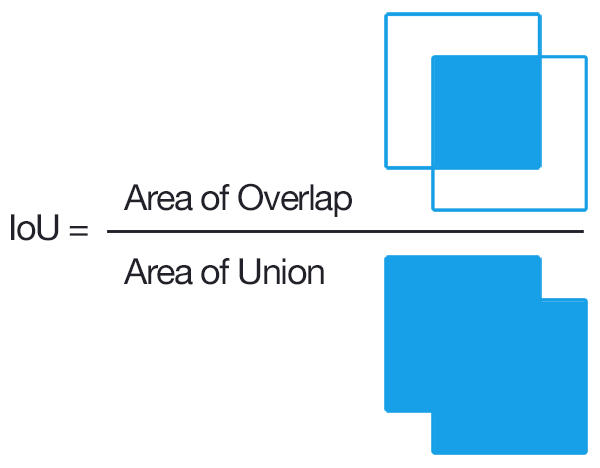
\includegraphics[width=0.4\textwidth]{images/011Fundamentals/IoU.png}
    \caption{Graphical Visualiziation for IoU. \cite{iou_pic}}
    \label{fig:IoU}
\end{figure}

Die \acrfull{IoU}, auch als Jaccard-Index bekannt, ist die am häufigsten verwendete Metrik zum Vergleich der Ähnlichkeit zweier beliebiger Formen. Sie kodiert die Formmerkmale der zu vergleichenden Objekte, beispielsweise Höhe, Breite und Position zweier \acrshort{BB}, in eine Bereichseigenschaft und berechnet daraus ein normalisiertes Maß, das sich auf die verglichenen Flächen oder Volumina bezieht (siehe Abb. \ref{fig:IoU}). Diese Eigenschaft macht die \acrshort{IoU} unabhängig von der Größe des betrachteten Objekts \cite{Rezatofighi2019}.

Aufgrund dieser Unabhängigkeit basiert eine Vielzahl von Leistungsmaßen in den Bereichen Segmentierung \cite{Ramirez2019,cordts2016,Zhou2017,lin2015}, Objekterkennung \cite{lin2015,Everingham2010} und Objektverfolgung \cite{Kristan2016,lealtaixé2015} auf der \acrshort{IoU}. Dabei entspricht eine der beiden \acrshort{BB} der Ground Truth, also dem korrekt gelabelten und lokalisierten Objekt, während die zweite \acrshort{BB} die vom Modell vorhergesagte Lokalisierung des Objektes darstellt. Die auf dieser Grundlage berechnete Übereinstimmung (\acrshort{IoU}), bei der die Überlappungsfläche der beiden Bounding Boxen durch die Gesamtfläche, die beide abdecken, geteilt wird, ermöglicht eine präzise Bewertung der Genauigkeit von Deep-Learning-Modellen.
\begin{definition}[Intersection over Union]
    Let $B_t$ be the set of image pixels covered by a Ground Truth Bounding Box for a class $k$, 
    and $B_p$ be the set of image pixels covered by a predicted Bounding Box for the same class. 
    Then the IoU is calculated as follows:

    \begin{equation}
    \text{IoU}_k =
    \begin{cases}
        \dfrac{|B_t \cap B_p|}{|B_t \cup B_p|}, & \text{if } |B_t \cup B_p| > 0, \\[6pt]
        0, & \text{otherwise.}
    \end{cases}
    \end{equation}

\end{definition}

% \begin{itemize}
%     \item \Acrfull{IoU}, oder auch Jaccard-Index, ist die am häufigsten verwendete Metrik zum Vergleich der Ähnlichkeit zweier beliebiger Formen
%     \item kodiert die Formmerkmale der vergleichenenden Objekte (z. B. Höhe, Breite und Positionen zweier \acrshort{BB}) in die Bereichseigenschaft und berechnet ein normalisiertes Maß, dass sich auf die verglichenen Flächen (oder Volumina) bezieht (s. Fig \ref{fig:IoU}); diese Eigenschaft macht \Acrshort{IoU} unabhängig von der Größe des betrachten Objekts \cite{Rezatofighi2019}
%     \item aufgrund dieser Eigenschaft basieren alle Leistungsmaße zur Bewertung von Segmentierung \cite{Ramirez2019,cordts2016,Zhou2017,lin2015}, Objekterkennung \cite{lin2015,Everingham2010} und -Verfolgung \cite{Kristan2016,lealtaixé2015} auf dieser Metrik
%     \item Dabei entspricht eine \Acrshort{BB} der Ground Truth, also dem gelabelten richtig verortetem Objekt, und die zweite \Acrshort{BB} der vom Modell vorhergesagten Lokalisierung des Objektes. Mit der daraus berechneten Übereinstimmung (\acrshort{IoU}) kann sich die Genauigkeit eines \Acrshort{DL} Modells bewerten.
% \end{itemize}






\subsection{Mean Average Precision (mAP)}

Die \acrlong{IoU} steht in engem Zusammenhang mit der \acrfull{mAP}, ist jedoch nicht identisch. Während die \acrshort{IoU} die Genauigkeit eines einzelnen vorhergesagten \acrshort{BB} misst, stellt die \acrshort{mAP} eine umfassendere Metrik dar, die die Leistung eines Modells über alle Objekte und Klassen eines Datensatzes bewertet \cite{ultralyics_iou}.

Zur Berechnung der \acrshort{mAP} werden die Konzepte Precision und Recall herangezogen. Precision beschreibt den Anteil der vom Modell als positiv klassifizierten Erkennungen, die tatsächlich korrekt sind, während Recall den Anteil der tatsächlich vorhandenen Objekte angibt, die korrekt erkannt wurden. Auf Basis dieser Werte kann eine \acrfull{PRC} (s. Def. \ref{Def:IPRC}) erstellt werden, wobei Precision auf der Y-Achse und Recall auf der X-Achse abgetragen wird \cite{Goodfellow-et-al-2016}. Objektdetektoren geben für jede Bounding Box eine Konfidenz an, die die Sicherheit des Modells hinsichtlich der Vorhersage widerspiegelt. Vorhersagen, deren Konfidenz unter einer festgelegten Schwelle liegen, können verworfen werden. 

\begin{definition}[Interpolated Precision-Recall Curve]
\label{Def:IPRC}
Let $P(r)$ be the value of precision at recall value $r$. 
The interpolation of the precision-recall curve is then given by $P_{int}$.

\begin{equation}
P_{int}(r) = \max_{r \leq y} P(y)
\end{equation}
\end{definition}


Die \acrshort{PRC} kann für alle möglichen Konfidenzschwellen erstellt werden, wodurch sich die durchschnittliche Präzision als Fläche unter der Kurve berechnen lässt. Die Modellbewertung erfolgt anschließend anhand der \acrfull{mAP} (s. Form. \ref{form:mAP}), die als Mittelwert der \acrfull{AP} (s. Form. \ref{form:AP}) über alle Klassen ermittelt wird (s. Def. \ref{Def:mAP})\cite{Rainio2024}. Dabei können unterschiedliche Genauigkeitsanforderungen an die Übereinstimmung der Bounding Boxes gestellt werden, beispielsweise durch IoU-Schwellenwerte von 0,5 oder einem Bereich von 0,5 bis 0,95. Letzteres entspricht dem Mittelwert von \acrshort{mAP}@0.5, \acrshort{mAP}@0.55 bis \acrshort{mAP}@0.95. Diese strengere Metrik erfordert eine größere Überlappung zwischen Ground Truth und Vorhersage und ist besonders geeignet, wenn die vorhergesagten Positionen der Bounding Boxes sehr präzise sein müssen \cite{Rainio2024}.


\begin{definition}[Mean Average Precision]
\label{Def:mAP}
Let $C$ be the set of classes with $c \in C$, and $P_{int}(r)$ be the interpolated precision-recall curve. 
The Average Precision (AP) and the mean Average Precision (mAP) are then defined as follows:

\begin{equation}
\label{form:AP}
AP_c = \int_0^1 P_{int}(r)\,dr
\end{equation}

\begin{equation}
\label{form:mAP}
mAP = \frac{1}{|C|} \sum_c AP_c
\end{equation}
\end{definition}

% \begin{itemize}
%     \item \Acrfull{IoU} ist mit \acrfull{mAP} verwandt aber nicht identisch
%     \item \acrshort{IoU} misst die Genauigkeit eines einzelnen vorhergesagten \acrshort{BB}, während \acrshort{mAP} eine umfassende Metrik ist, die die Leistung eines Modells über alle Objekte udn Klassen in einem Datensatz berechnet \cite{ultralyics_iou}
% \end{itemize}
% \begin{itemize}
%     \item Precision ist der Anteil der vom Modell gemeldeteten Erkennungen, die korrekt waren 
%     \item Recall der Anteil an Erkennungen der tatsächlich aufgetretenen Objekte, die erkannt wurden
%     \item \Acrfull{PRC} kann gezeichnet werden, wobei Precision auf Y und Recall auf X Achse dargestellt wird \cite{Goodfellow-et-al-2016}
%     \item Objektdetektor gibt für jede BB eine Konfidenz aus, die angibt, wie sicher sich das Modell hinsichtlich der Vorhersage ist
%     \item Vorhersagen unterhalb einer bestimmten Konfidenzschwelle können entfernt werden
%     \item \acrshort{PRC} kann man auch bei allen möglichen Konfidenzschwellen  erstellen, dann kann man die durchschnittliche Präzision als Fläche unter der \acrshort{PRC} berechnen
%     \item Modellbewertung anhand der \Acrfull{mAP}, die als Mittelwert der \Acrfull{AP} in allen verschiedenen Klassen berechnet wird \cite{Rainio2024}
%     \item Verschiedene Genauigkeiten bei der Übereinstimmung möglich, bei IoU Schwellwert von 0.5 oder auch von 0.5-0.95. Letzteres entspricht dem Mittelwert von \Acrshort{mAP}@0.5, \acrshort{mAP}@0.55, .. , \Acrshort{mAP}@0.95. Das ist eine strengere Metrik, da Sie eine größere Überlappung für potenzielle Übereinstimmungen erfordert und aus diesem Grund ist diese Metrik gut für Situationen geeignet, in denen die vorhergesagten Positionen der BB sehr genau sein müssen \cite{Rainio2024}
% \end{itemize}





